
% fill=gray!50

\begin{figure}[t!]%h!
    \centering
    \begin{subfigure}{.47\textwidth}
        \centering
        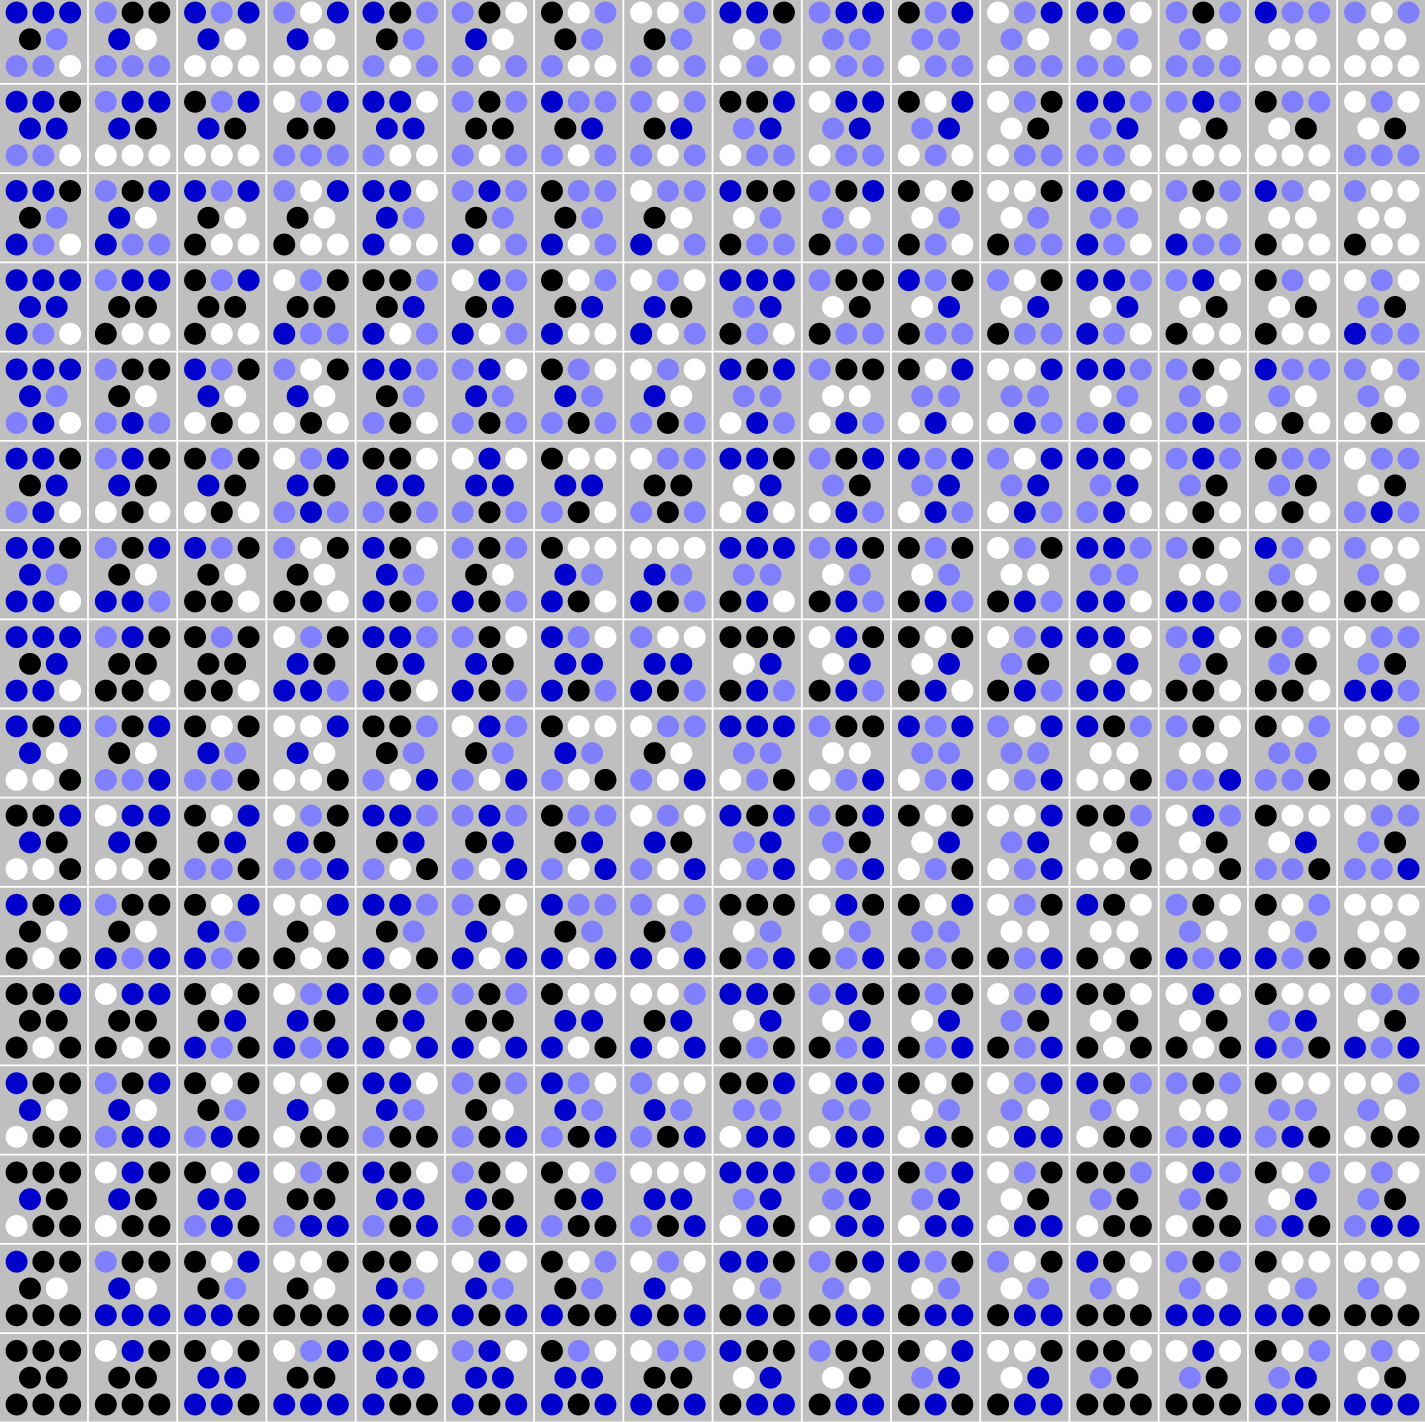
\includegraphics[width=0.9\linewidth]{keller_clique.png}
        %* —————————————————
        \caption{A Keller graph \cite{brakensiekResolutionKellerConjecture2020}}
        \label{fig:tiling_seven}
    \end{subfigure}\quad
    \begin{subfigure}{.47\textwidth}
        \centering
        %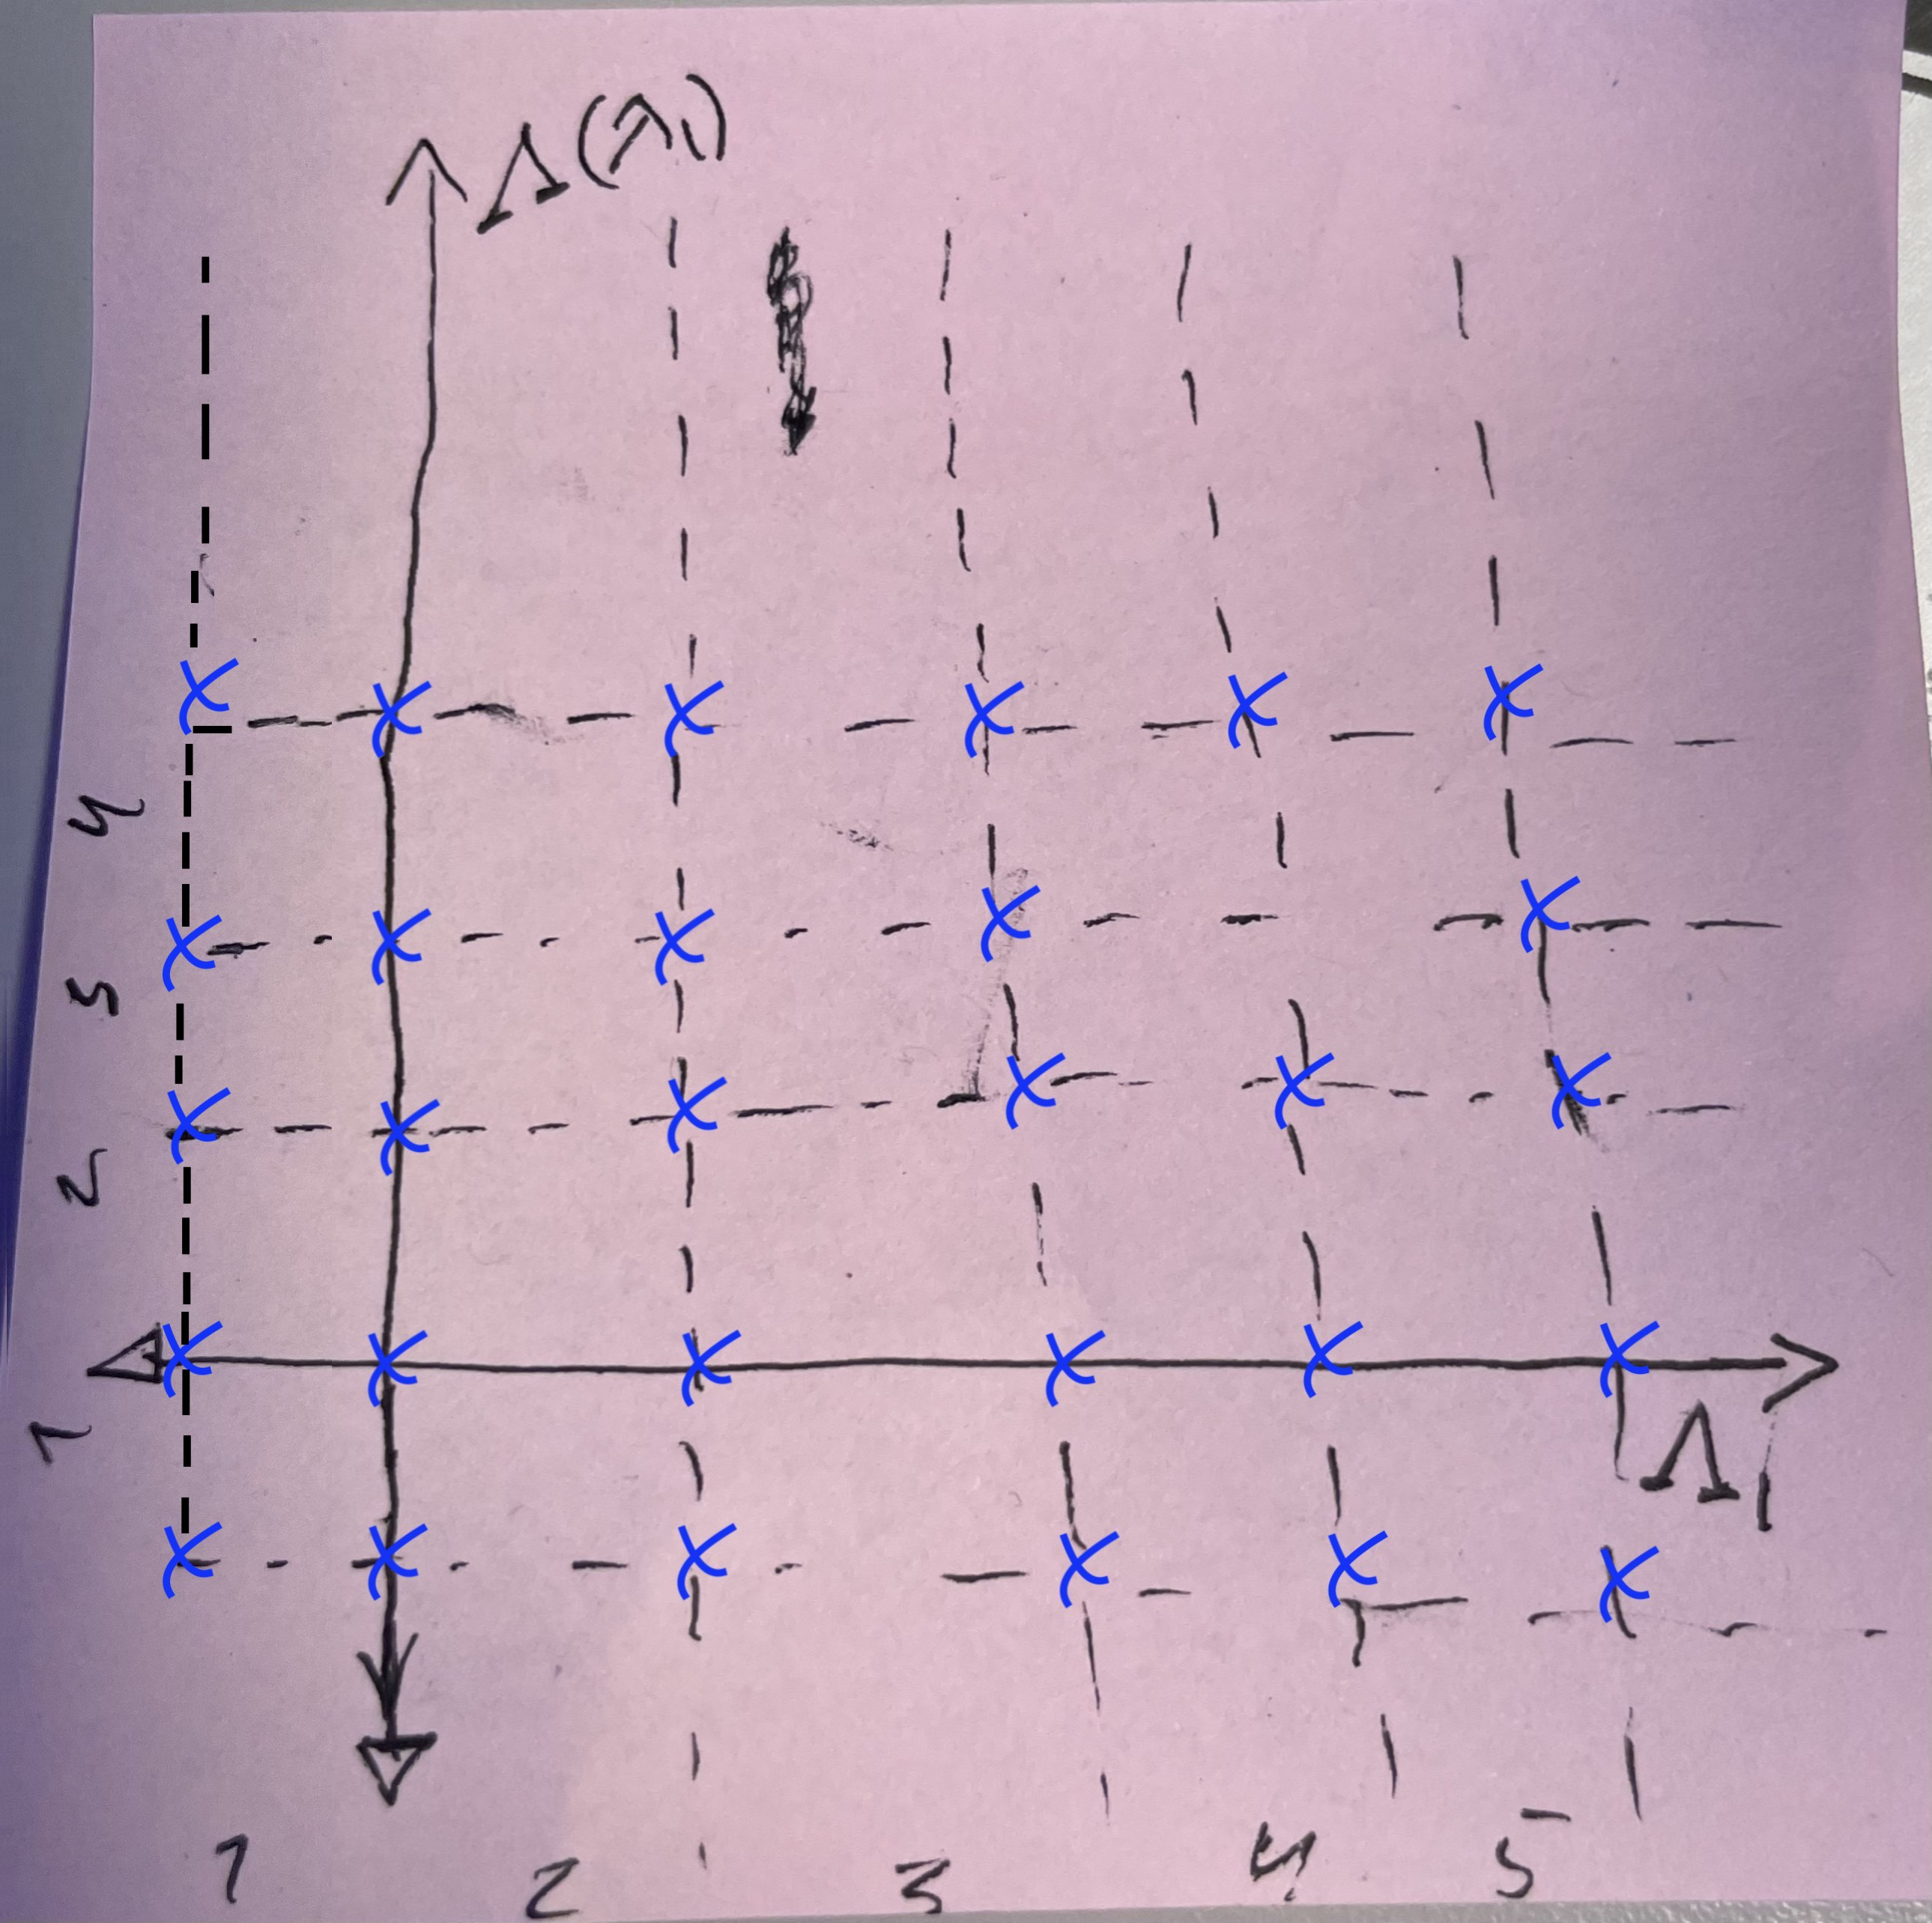
\includegraphics[width=0.9\linewidth]{spec_no_shift.jpg}
        %* Figure 1              
        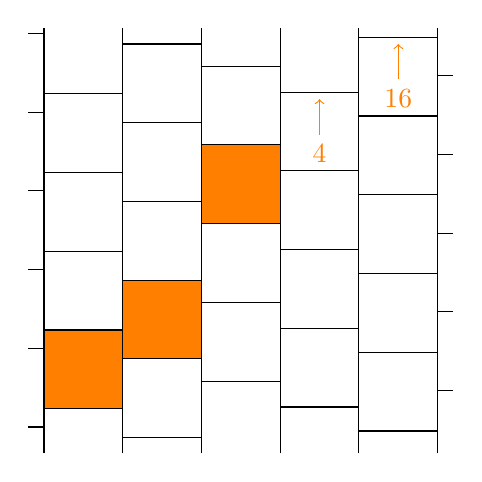
\begin{tikzpicture}[scale=1]
            % Define the tile
            \def\tile{
            % Draw the unit square
            \draw[fill=white] (0,0) rectangle (1,1);
            }
            \def\tiletwo{
            %\draw[fill=gray!65] (0,0) rectangle (1,1);
            \draw[fill=orange] (0,0) rectangle (1,1);
            %\draw[->] (0.5,0) -- (0.5,0.9);  % If arrows from the middle
            }
            % Right border tile
            \def\tileThree{
            %\draw[fill=red] (0,0) rectangle (1,1);  % test tile to se if we got the right one
            \draw[black] (0,1) -- (0+0.2,1);  % Right_top
            \draw[black] (0,0) -- (0+0.2,0);  % Right_bottom
            }
            % Left border tile
            \def\tileFour{
            % If using test square, must change from x=0 to x=1 for the left border markers
            %\draw[fill=red] (0,0) rectangle (1,1);  % test tile to se if we got the right one
            \draw[black] (0,1) -- (0-0.2,1);  % Right_top
            \draw[black] (0,0) -- (0-0.2,0);  % Right_bottom
            }
            
            % Exponential function parameters
            \pgfmathsetmacro{\base}{2} % Base of the exponential function
            \pgfmathsetmacro{\expMinTwo}{exp(-2)}
            \pgfmathsetmacro{\expMinOne}{exp(-1)}
            \pgfmathsetmacro{\expZero}{exp(0)}
            \pgfmathsetmacro{\expOne}{exp(1)}
            \pgfmathsetmacro{\expTwo}{exp(2)}
            \pgfmathsetmacro{\expThree}{exp(3)}
            \pgfmathsetmacro{\expFour}{exp(4)}

            % Shift list
            \def\BetaMinOne{\expMinOne}
            \def\BetaZero{\expZero}
            \def\BetaOne{\expOne}
            \def\BetaTwo{\expTwo}
            \def\BetaThree{\expThree}
            \def\BetaFour{\expFour}

            % Left border markers
            \foreach \x in {0}{
                \foreach \y in {0,1,2,3,4}{
                    \pgfmathsetmacro{\shiftX}{\x}
                    \pgfmathsetmacro{\shiftY}{\y + \expMinTwo}
                    \pgfmathsetmacro{\shiftSingle}{\expMinTwo}
                    
                    % Drawing the rest of the middle cubes
                    \begin{scope}[shift={(\shiftX,\shiftY)}]
                        \tileFour
                    \end{scope}
        }}
            % Right border markers
            \foreach \x in {5}{
                \foreach \y in {-54,...,-51}{
                    \pgfmathsetmacro{\shiftX}{\x}
                    \pgfmathsetmacro{\shiftY}{\y + \BetaFour}
                    \pgfmathsetmacro{\shiftSingle}{\BetaFour}
                    % Drawing the rest of the middle cubes
                    \begin{scope}[shift={(\shiftX,\shiftY)}]
                        \tileThree
                    \end{scope}
                    
        }}


            % Draw the tiling pattern Latter part
            \foreach \x in {1}{
                \foreach \y in {-1,...,3}{
                    \pgfmathsetmacro{\shiftX}{\x}
                    \pgfmathsetmacro{\shiftY}{\y + \BetaZero}
                    \pgfmathsetmacro{\shiftSingle}{\BetaZero}
                    % Drawing the rest of the middle cubes
                    \begin{scope}[shift={(\shiftX,\shiftY)}]
                        \tile
                    \end{scope}
                    % No need for orange cubes as they would be outside
                }}
            \foreach \x in {2}{
                \foreach \y in {-2,...,1}{
                    \pgfmathsetmacro{\shiftX}{\x} 
                    \pgfmathsetmacro{\shiftY}{\y + \BetaOne} 
                    \pgfmathsetmacro{\shiftSingle}{0+\BetaOne}
                    % Drawing the rest of the middle cubes
                    \begin{scope}[shift={(\shiftX,\shiftY)}]
                        \tile
                    \end{scope}
                    % No need for orange cubes as they would be outside
                }}
            \foreach \x in {3}{
                \foreach \y in {-7,...,-4}{
                    \pgfmathsetmacro{\shiftX}{\x}
                    \pgfmathsetmacro{\shiftY}{\y + \BetaTwo}
                    \pgfmathsetmacro{\shiftSingle}{\BetaTwo}
                    % Drawing the rest of the middle cubes
                    \begin{scope}[shift={(\shiftX,\shiftY)}]
                        \tile
                    \end{scope}
                    % No need for orange cubes as they would be outside
                    % REMEMBER that we have shifted the entirety of what is plotted from this column, 
                    % our grid is still x: -1,...,5 and   y: 0,...,4 i.e., The leftmost markers!!                  
                    \ifnum\y=-4
                        \draw[->, orange] (\x+0.5,3.85) node[below] {$4$} -- (\x+0.5,4.3);
                    \fi
                }}
                \foreach \x in {4}{
                    \foreach \y in {-20,...,-16}{
                    \pgfmathsetmacro{\shiftX}{\x}
                    \pgfmathsetmacro{\shiftY}{\y + \BetaThree}
                    \pgfmathsetmacro{\shiftSingle}{\BetaThree}
                    % Drawing the rest of the middle cubes
                    \begin{scope}[shift={(\shiftX,\shiftY)}]
                        \tile
                    \end{scope}
                    % No need for orange cubes as they would be outside
                    % REMEMBER that we have shifted the entirety of what is plotted from this column, 
                    % our grid is still x: -1,...,5 and   y: 0,...,4 i.e., The leftmost markers!!               
                    \ifnum\y=-16
                        \draw[->, orange] (\x+0.5,4.55) node[below] {$16$} -- (\x+0.5,5);
                    \fi
                }}
                
            % Draw the tiling pattern
            \foreach \x in {0}{
                \foreach \y in {0,1,2,3}{
                    \pgfmathsetmacro{\shiftX}{\x}
                    \pgfmathsetmacro{\shiftY}{\y + \BetaMinOne}
                    \pgfmathsetmacro{\shiftSingle}{0+\BetaMinOne}
                    % Drawing the rest of the middle cubes
                    \begin{scope}[shift={(\shiftX,\shiftY)}]
                        \tile
                    \end{scope}
                }  
            }
            
            % Orange cube overlay
            \foreach \x in {0,1,2}{
                \foreach \y in {0,1,2,3}{
                    \ifnum\x=0
                        \pgfmathsetmacro{\shiftX}{\x}
                        \pgfmathsetmacro{\shiftY}{\y + \BetaMinOne}
                        \pgfmathsetmacro{\shiftSingle}{0+\BetaMinOne}
                    \fi
                    \ifnum\x=1
                        \pgfmathsetmacro{\shiftX}{\x}
                        \pgfmathsetmacro{\shiftY}{\y + \BetaZero}
                        \pgfmathsetmacro{\shiftSingle}{0+\BetaZero}
                    \fi
                    \ifnum\x=2
                        \pgfmathsetmacro{\shiftX}{\x}
                        \pgfmathsetmacro{\shiftY}{\y + \BetaOne}
                        \pgfmathsetmacro{\shiftSingle}{0+\BetaOne}
                    \fi
                    % Drawing a new line of shifted colored cubes on top at the first row
                    \ifnum\y=0
                        \begin{scope}[shift={(\shiftX,\shiftY)}]
                            \tiletwo
                        \end{scope}
                    \fi
        }}
            % get the outline grid 
            % Whole black lines
            \foreach \x in {0,1,2,3,4,5}{
                \draw (\x,0-0.2) -- (\x,5+0.2);  % Shift only in the vertical direction, therefore only one line
            }
        \end{tikzpicture}
        %* —————————————————
        \caption{Non-periodic tiling of unit cubes}
        \label{fig:tiling_eight}
    \end{subfigure}
    \caption{Illustrated in \cref{fig:tiling_seven} is a clique of size $2^8=256$ in the Keller graph of $G_{8,2}$, which disproves Keller's \namecref{conj:keller_tiling} for $d\geq8$. Each grey square of $8$ dots represents a vertex, and each dot inside the square represents a coordinate. The coordinate set in the Keller graph of $G_{8,2}$ is $\braq{0,1,2,3}$, where the colors black, dark blue, white, or light blue respectively represents each of the possible coordinate values. Observe that for the vertices to be adjacent, it is enough for any two vertices to have a complimentary dot, which means either black versus white or dark blue versus light blue; \textsc{and} at least one dot of a different color as a different color represents a different coordinate. Illustrated in \cref{fig:tiling_eight} is a non-periodic tiling with unit cubes of $\R^2$ where the $n$'th column of unit cubes is shifted in the vertical direction by the value of $e^n$, for all $n\in\Z$. The arrow with an orange number indicates the number of unit squares from the arrow to the orange-colored unit square. If this were a lattice tiling, all orange-colored squares would be on the same horizontal line. The line fragments of the $-2$'th and $4$'th columns of unit cubes can be observed at the left and right edges, respectively.}
    \label{fig:tilings_seven_eight}
\end{figure}